% Source: graduate-coursework/Sp26/CSCE775/course_notes/mc_action_values_guide.tex

\documentclass[border=4pt]{standalone}
\usepackage{amsfonts}
\usepackage{amsmath}
\usepackage{amssymb}
\usepackage{amsthm}
\usepackage[T1]{fontenc}
\usepackage{graphicx}
\usepackage{tikz}
\usepackage{xcolor}
\usetikzlibrary{arrows.meta, positioning, shapes.geometric, calc, decorations.pathreplacing}

\definecolor{Garnet}{HTML}{73000a}
\definecolor{SecondaryBlue}{HTML}{466A9F}
\definecolor{SecondaryGreen}{HTML}{65780B}
\definecolor{FlatRed}{HTML}{CC2E40}
\definecolor{FlatDark}{HTML}{1F414D}
\definecolor{FlatYellow}{HTML}{CED318}
\definecolor{FlatGold}{HTML}{A49137}
\definecolor{LightGray}{HTML}{F0F0F0}
\definecolor{Rose}{HTML}{CC2E40}

\renewcommand{\baselinestretch}{1.2}
\newcommand{\vocab}[1]{\textbf{\textcolor{Garnet}{#1}}}
\newcommand{\mathhighlight}[1]{\textcolor{SecondaryBlue}{#1}}

\begin{document}
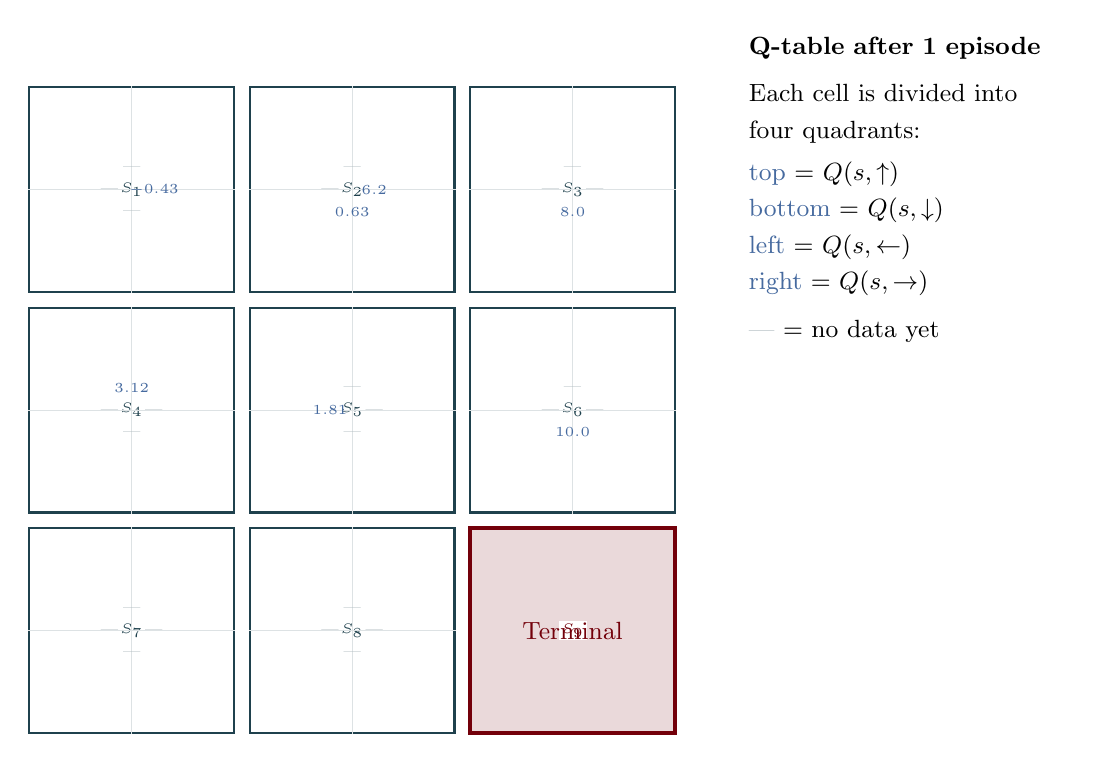
\begin{tikzpicture}[
    cell/.style={minimum size=2.6cm, draw=FlatDark, thick},
    goal/.style={cell, fill=Garnet!15, draw=Garnet, line width=1.5pt},
    empty/.style={cell, fill=LightGray},
    qval/.style={font=\tiny\bfseries, SecondaryBlue},
    qempty/.style={font=\tiny, FlatDark!35},
    slabel/.style={font=\tiny, FlatDark, fill=white, inner sep=1pt}
]
\def\cellspacing{2.8}
% Draw all 9 cells
\foreach \row/\rowidx in {2/0, 1/1, 0/2} {
    \foreach \col/\colidx in {0/0, 1/1, 2/2} {
        \pgfmathtruncatemacro{\idx}{\rowidx*3+\colidx+1}
        \ifnum\idx=9
            \node[goal] (s\idx) at (\col*\cellspacing, \row*\cellspacing) {};
        \else
            \node[cell] (s\idx) at (\col*\cellspacing, \row*\cellspacing) {};
        \fi
        % State label in center
        \ifnum\idx=9
            \node[slabel] at (s\idx.center) {\textcolor{Garnet}{$S_{\idx}$}};
        \else
            \node[slabel] at (s\idx.center) {$S_{\idx}$};
        \fi
        % Cross lines
        \ifnum\idx<9
            \draw[FlatDark!15] ([xshift=0pt]s\idx.west) -- ([xshift=0pt]s\idx.east);
            \draw[FlatDark!15] ([yshift=0pt]s\idx.south) -- ([yshift=0pt]s\idx.north);
        \fi
    }
}

% Q-values for S1: Right = -0.43
\node[qempty] at ([yshift=8pt]s1.center) {---};
\node[qempty] at ([yshift=-8pt]s1.center) {---};
\node[qempty] at ([xshift=-8pt]s1.center) {---};
\node[qval] at ([xshift=8pt]s1.center) {$-0.43$};

% Q-values for S2: Down = 0.63, Right = 6.2
\node[qempty] at ([yshift=8pt]s2.center) {---};
\node[qval] at ([yshift=-8pt]s2.center) {$0.63$};
\node[qempty] at ([xshift=-8pt]s2.center) {---};
\node[qval] at ([xshift=8pt]s2.center) {$6.2$};

% Q-values for S3: Down = 8.0
\node[qempty] at ([yshift=8pt]s3.center) {---};
\node[qval] at ([yshift=-8pt]s3.center) {$8.0$};
\node[qempty] at ([xshift=-8pt]s3.center) {---};
\node[qempty] at ([xshift=8pt]s3.center) {---};

% Q-values for S4: Up = 3.12
\node[qval] at ([yshift=8pt]s4.center) {$3.12$};
\node[qempty] at ([yshift=-8pt]s4.center) {---};
\node[qempty] at ([xshift=-8pt]s4.center) {---};
\node[qempty] at ([xshift=8pt]s4.center) {---};

% Q-values for S5: Left = 1.81
\node[qempty] at ([yshift=8pt]s5.center) {---};
\node[qempty] at ([yshift=-8pt]s5.center) {---};
\node[qval] at ([xshift=-8pt]s5.center) {$1.81$};
\node[qempty] at ([xshift=8pt]s5.center) {---};

% Q-values for S6: Down = 10.0
\node[qempty] at ([yshift=8pt]s6.center) {---};
\node[qval] at ([yshift=-8pt]s6.center) {$10.0$};
\node[qempty] at ([xshift=-8pt]s6.center) {---};
\node[qempty] at ([xshift=8pt]s6.center) {---};

% S7, S8: all empty
\node[qempty] at ([yshift=8pt]s7.center) {---};
\node[qempty] at ([yshift=-8pt]s7.center) {---};
\node[qempty] at ([xshift=-8pt]s7.center) {---};
\node[qempty] at ([xshift=8pt]s7.center) {---};

\node[qempty] at ([yshift=8pt]s8.center) {---};
\node[qempty] at ([yshift=-8pt]s8.center) {---};
\node[qempty] at ([xshift=-8pt]s8.center) {---};
\node[qempty] at ([xshift=8pt]s8.center) {---};

% S9: terminal
\node[font=\small, Garnet] at (s9.center) {Terminal};

% Legend
\node[anchor=west, font=\small, text width=4cm] at ([xshift=0.8cm]s3.east) {
    \textbf{Q-table after 1 episode}\\[4pt]
    Each cell is divided into\\
    four quadrants:\\[2pt]
    \textcolor{SecondaryBlue}{top} = $Q(s,\uparrow)$\\
    \textcolor{SecondaryBlue}{bottom} = $Q(s,\downarrow)$\\
    \textcolor{SecondaryBlue}{left} = $Q(s,\leftarrow)$\\
    \textcolor{SecondaryBlue}{right} = $Q(s,\rightarrow)$\\[4pt]
    \textcolor{FlatDark!35}{---} = no data yet
};
\end{tikzpicture}
\end{document}
